\section{Interface}
\subsection{Master module}

Hình dưới đây là sơ đồ tổng khối của module Master, thể hiện các module con và kết nối giữa chúng.
\begin{figure}[H]
	\centering
	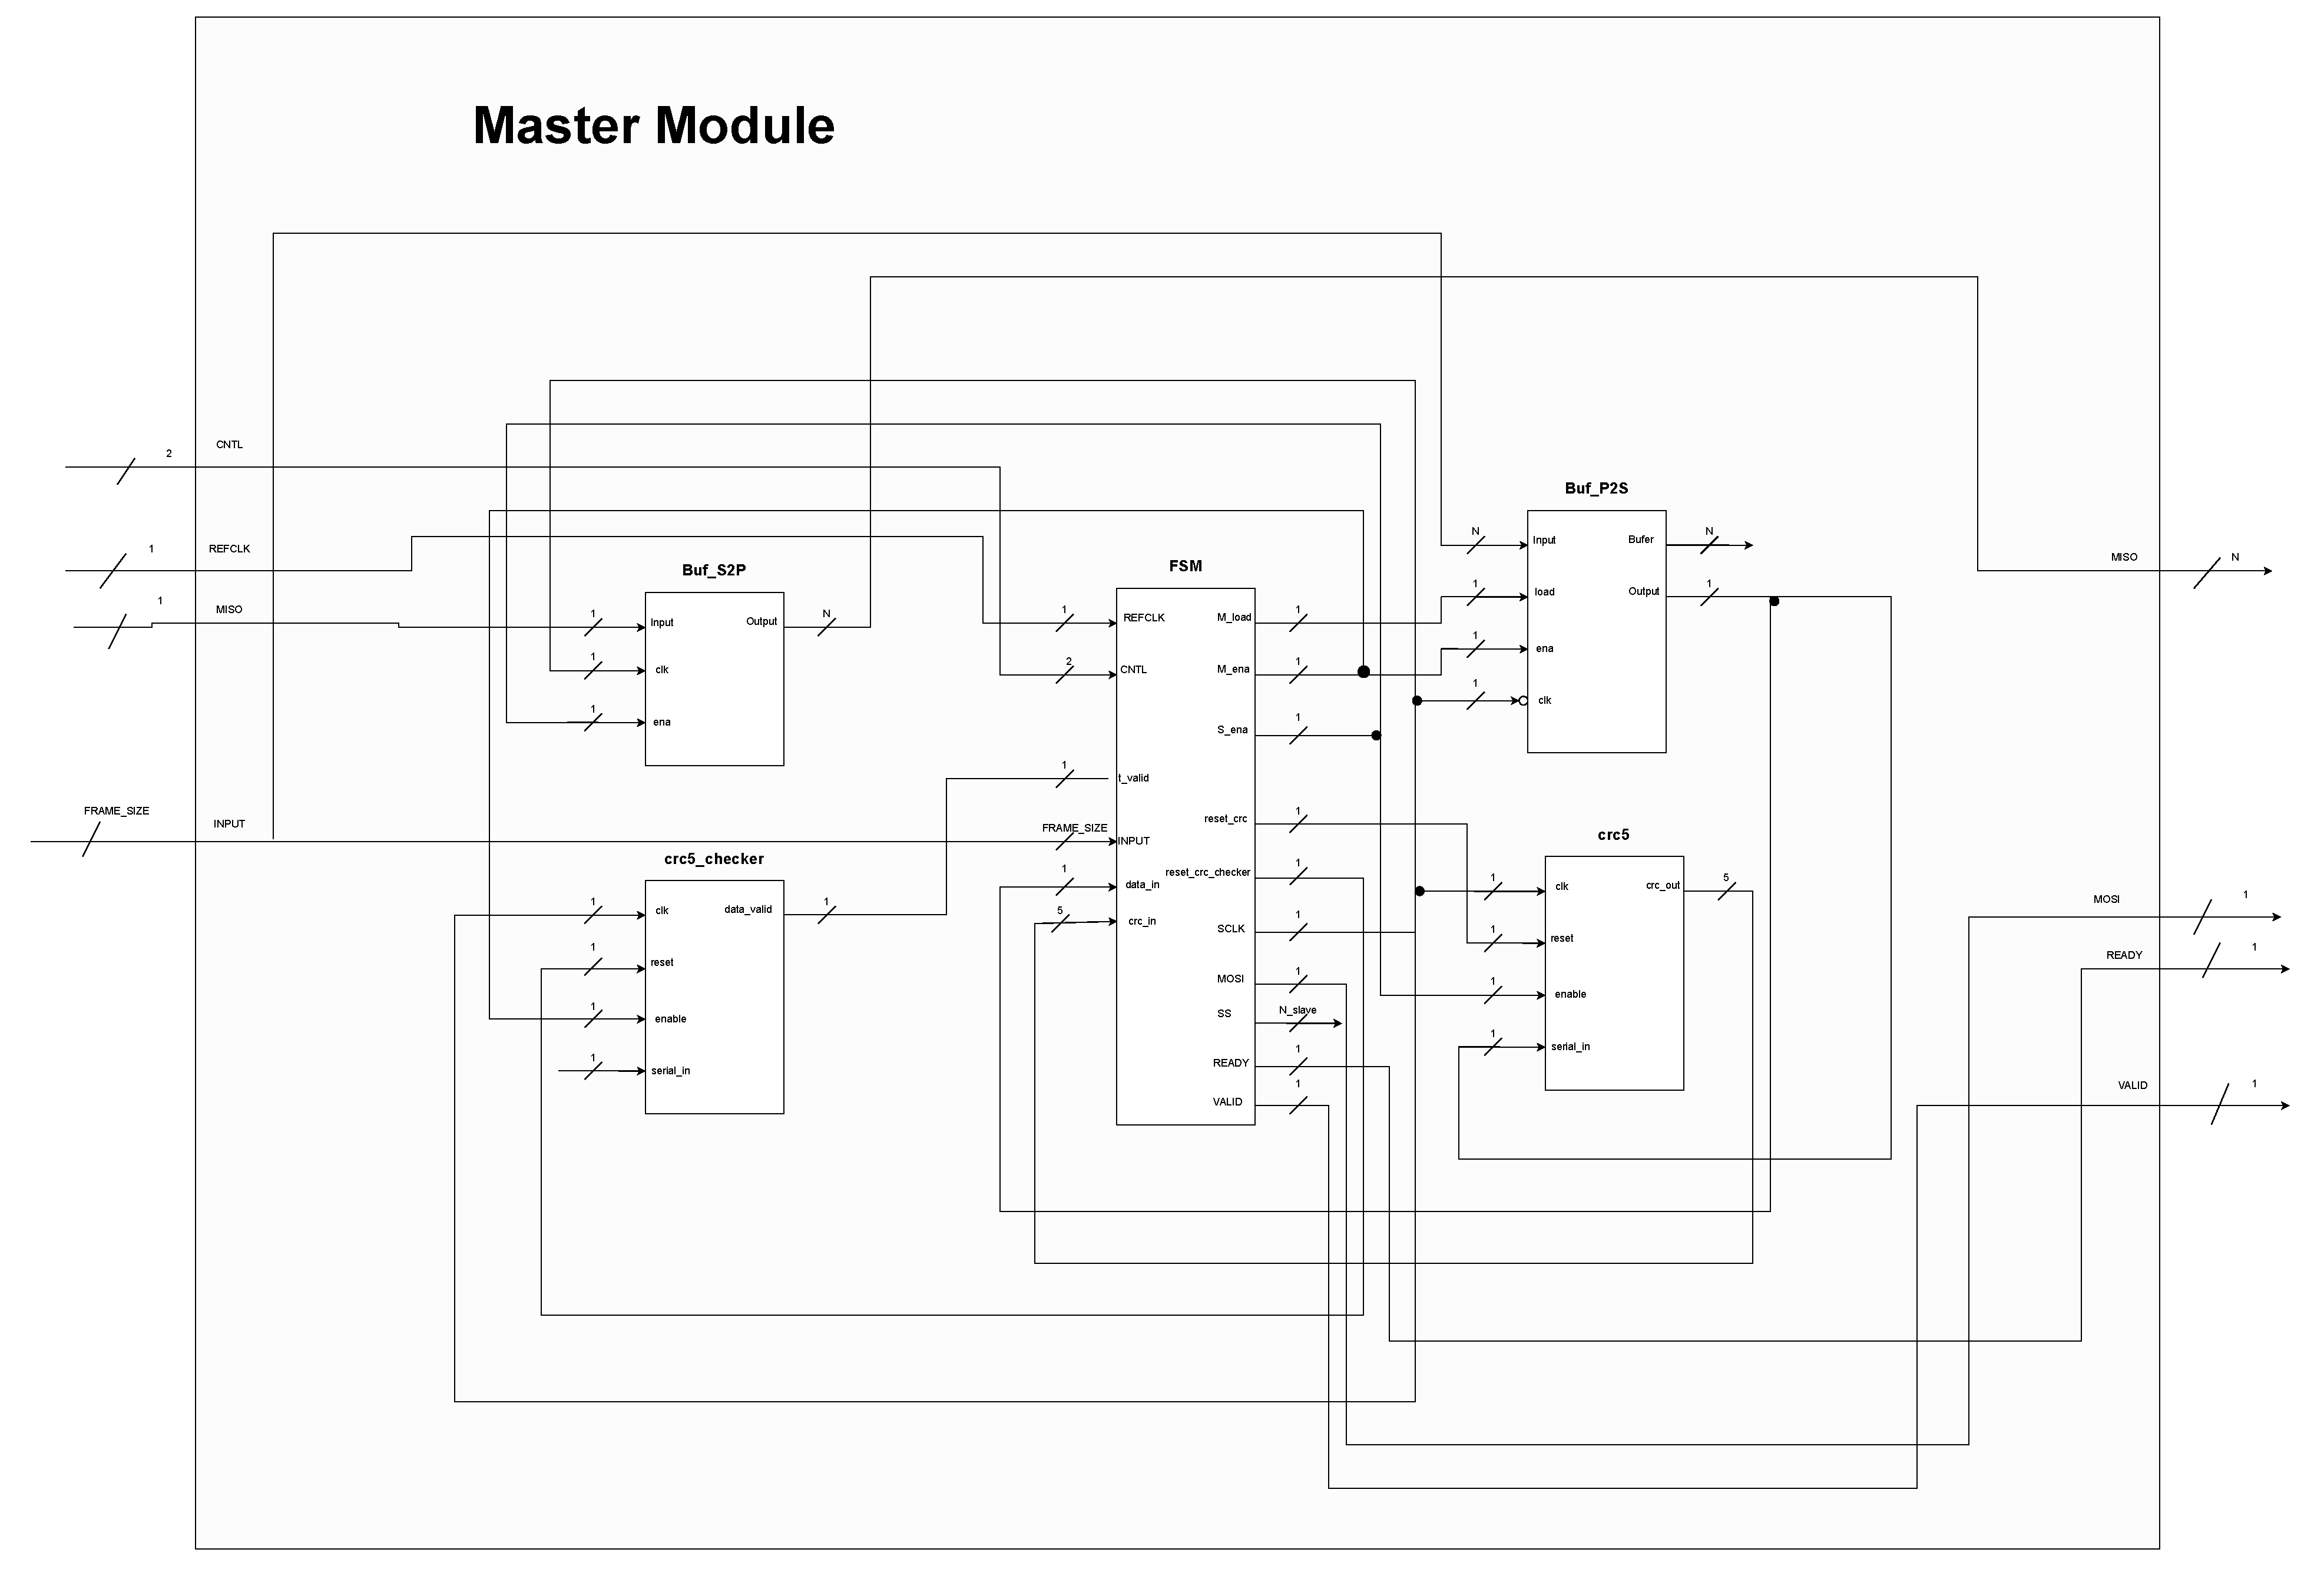
\includegraphics[width=0.85\textwidth]{graphics/Tai_5.pdf}
	\caption{Sơ đồ tổng khối Master}
	\label{fig:master_top}
\end{figure}
Các module con chính gồm: \texttt{Buf\_P2S}, \texttt{Buf\_S2P}, \texttt{crc5} và \texttt{crc5\_checker}.
\begin{figure}[H]
	\centering
	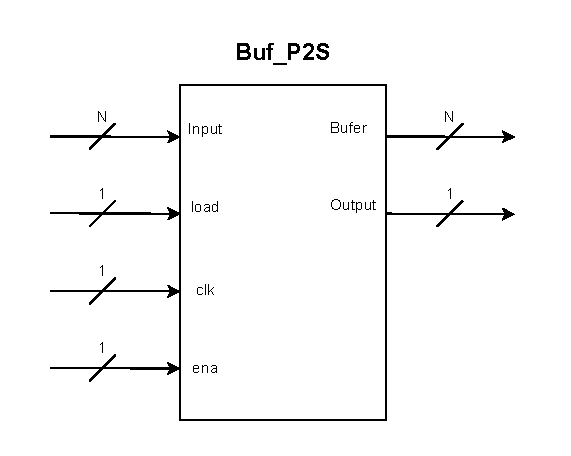
\includegraphics[width=0.6\textwidth]{graphics/Tai_1.pdf}
	\caption{Buf\_P2S}
	\label{fig:buf_p2s}
\end{figure}

\subsubsection*{Buf\_P2S}
\textbf{Tham số:} \texttt{N = 8} (mặc định).\\
\textbf{Cổng vào:}
\begin{itemize}
	\item \texttt{Input[N-1:0]}: dữ liệu song song đầu vào (N bit).
	\item \texttt{load}: tín hiệu nạp dữ liệu vào buffer.
	\item \texttt{clk}: xung đồng bộ cho dịch dữ liệu.
	\item \texttt{ena}: cho phép dịch.
\end{itemize}
\textbf{Cổng ra:}
\begin{itemize}
	\item \texttt{Output}: dữ liệu nối tiếp đầu ra (1 bit).
	\item \texttt{Buffer[N-1:0]}: nội dung buffer ở dạng song song.
\end{itemize}

\begin{figure}[H]
	\centering
	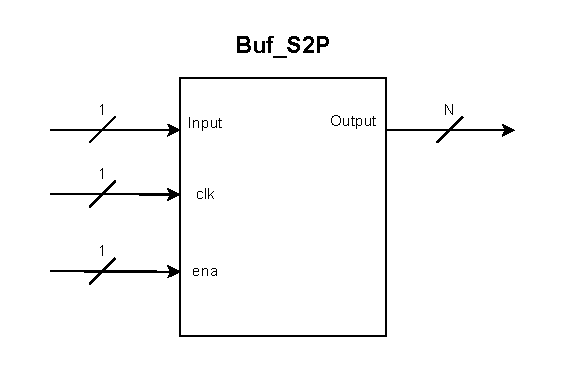
\includegraphics[width=0.6\textwidth]{graphics/Tai_2.pdf}
	\caption{Buf\_S2P}
	\label{fig:buf_s2p}
\end{figure}

\subsubsection*{Buf\_S2P}
\textbf{Tham số:} \texttt{N = 8} (mặc định).\\
\textbf{Cổng vào:}
\begin{itemize}
	\item \texttt{Input}: dữ liệu nối tiếp đầu vào (1 bit).
	\item \texttt{clk}: xung đồng bộ.
	\item \texttt{ena}: cho phép dịch.
\end{itemize}
\textbf{Cổng ra:}
\begin{itemize}
	\item \texttt{Output[N-1:0]}: dữ liệu song song sau khi thu đủ N bit.
\end{itemize}

\begin{figure}[H]
	\centering
	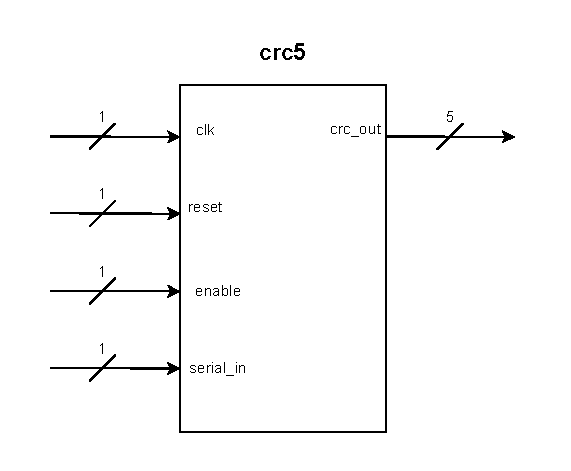
\includegraphics[width=0.6\textwidth]{graphics/Tai_3.pdf}
	\caption{crc5}
	\label{fig:crc5}
\end{figure}

\subsubsection*{crc5}
\textbf{Cổng vào:}
\begin{itemize}
	\item \texttt{clk}: xung đồng bộ.
	\item \texttt{reset}: đặt lại CRC về 0.
	\item \texttt{enable}: cho phép cập nhật CRC.
	\item \texttt{serial\_in}: dữ liệu nối tiếp đầu vào (1 bit).
\end{itemize}
\textbf{Cổng ra:}
\begin{itemize}
	\item \texttt{crc\_out[4:0]}: giá trị CRC-5 hiện tại.
\end{itemize}

\begin{figure}[H]
	\centering
	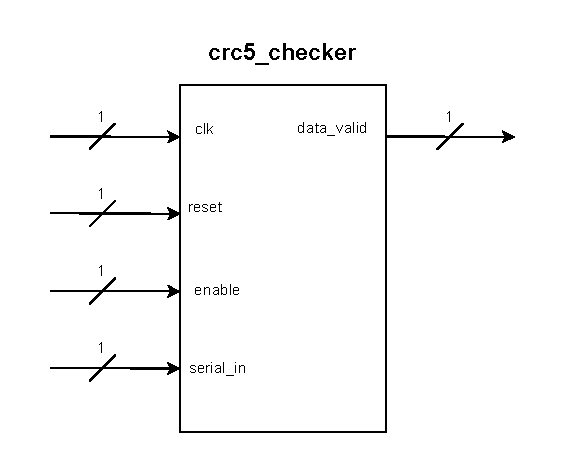
\includegraphics[width=0.6\textwidth]{graphics/Tai_4.pdf}
	\caption{crc5\_checker}
	\label{fig:crc5_checker}
\end{figure}

\subsubsection*{crc5\_checker}
\textbf{Cổng vào:}
\begin{itemize}
	\item \texttt{clk}: xung đồng bộ.
	\item \texttt{reset}: đặt lại bộ kiểm tra.
	\item \texttt{enable}: cho phép cập nhật CRC theo chuỗi nhận.
	\item \texttt{serial\_in}: dữ liệu nối tiếp đầu vào (1 bit).
\end{itemize}
\textbf{Cổng ra:}
\begin{itemize}
	\item \texttt{data\_valid}: báo dữ liệu hợp lệ khi CRC đúng.
	\item \texttt{check\_crc\_out[4:0]}: giá trị CRC đang kiểm tra (nếu cần quan sát).
\end{itemize}

\subsection{Slave module}
Khối chính là \texttt{SPI\_Slave\_CRC}, bên trong sử dụng các module con \texttt{Parallel\_to\_serial}, \texttt{serial\_to\_parallel}, \texttt{crc5} và \texttt{crc5\_checker}.
\begin{figure}[H]
	\centering
	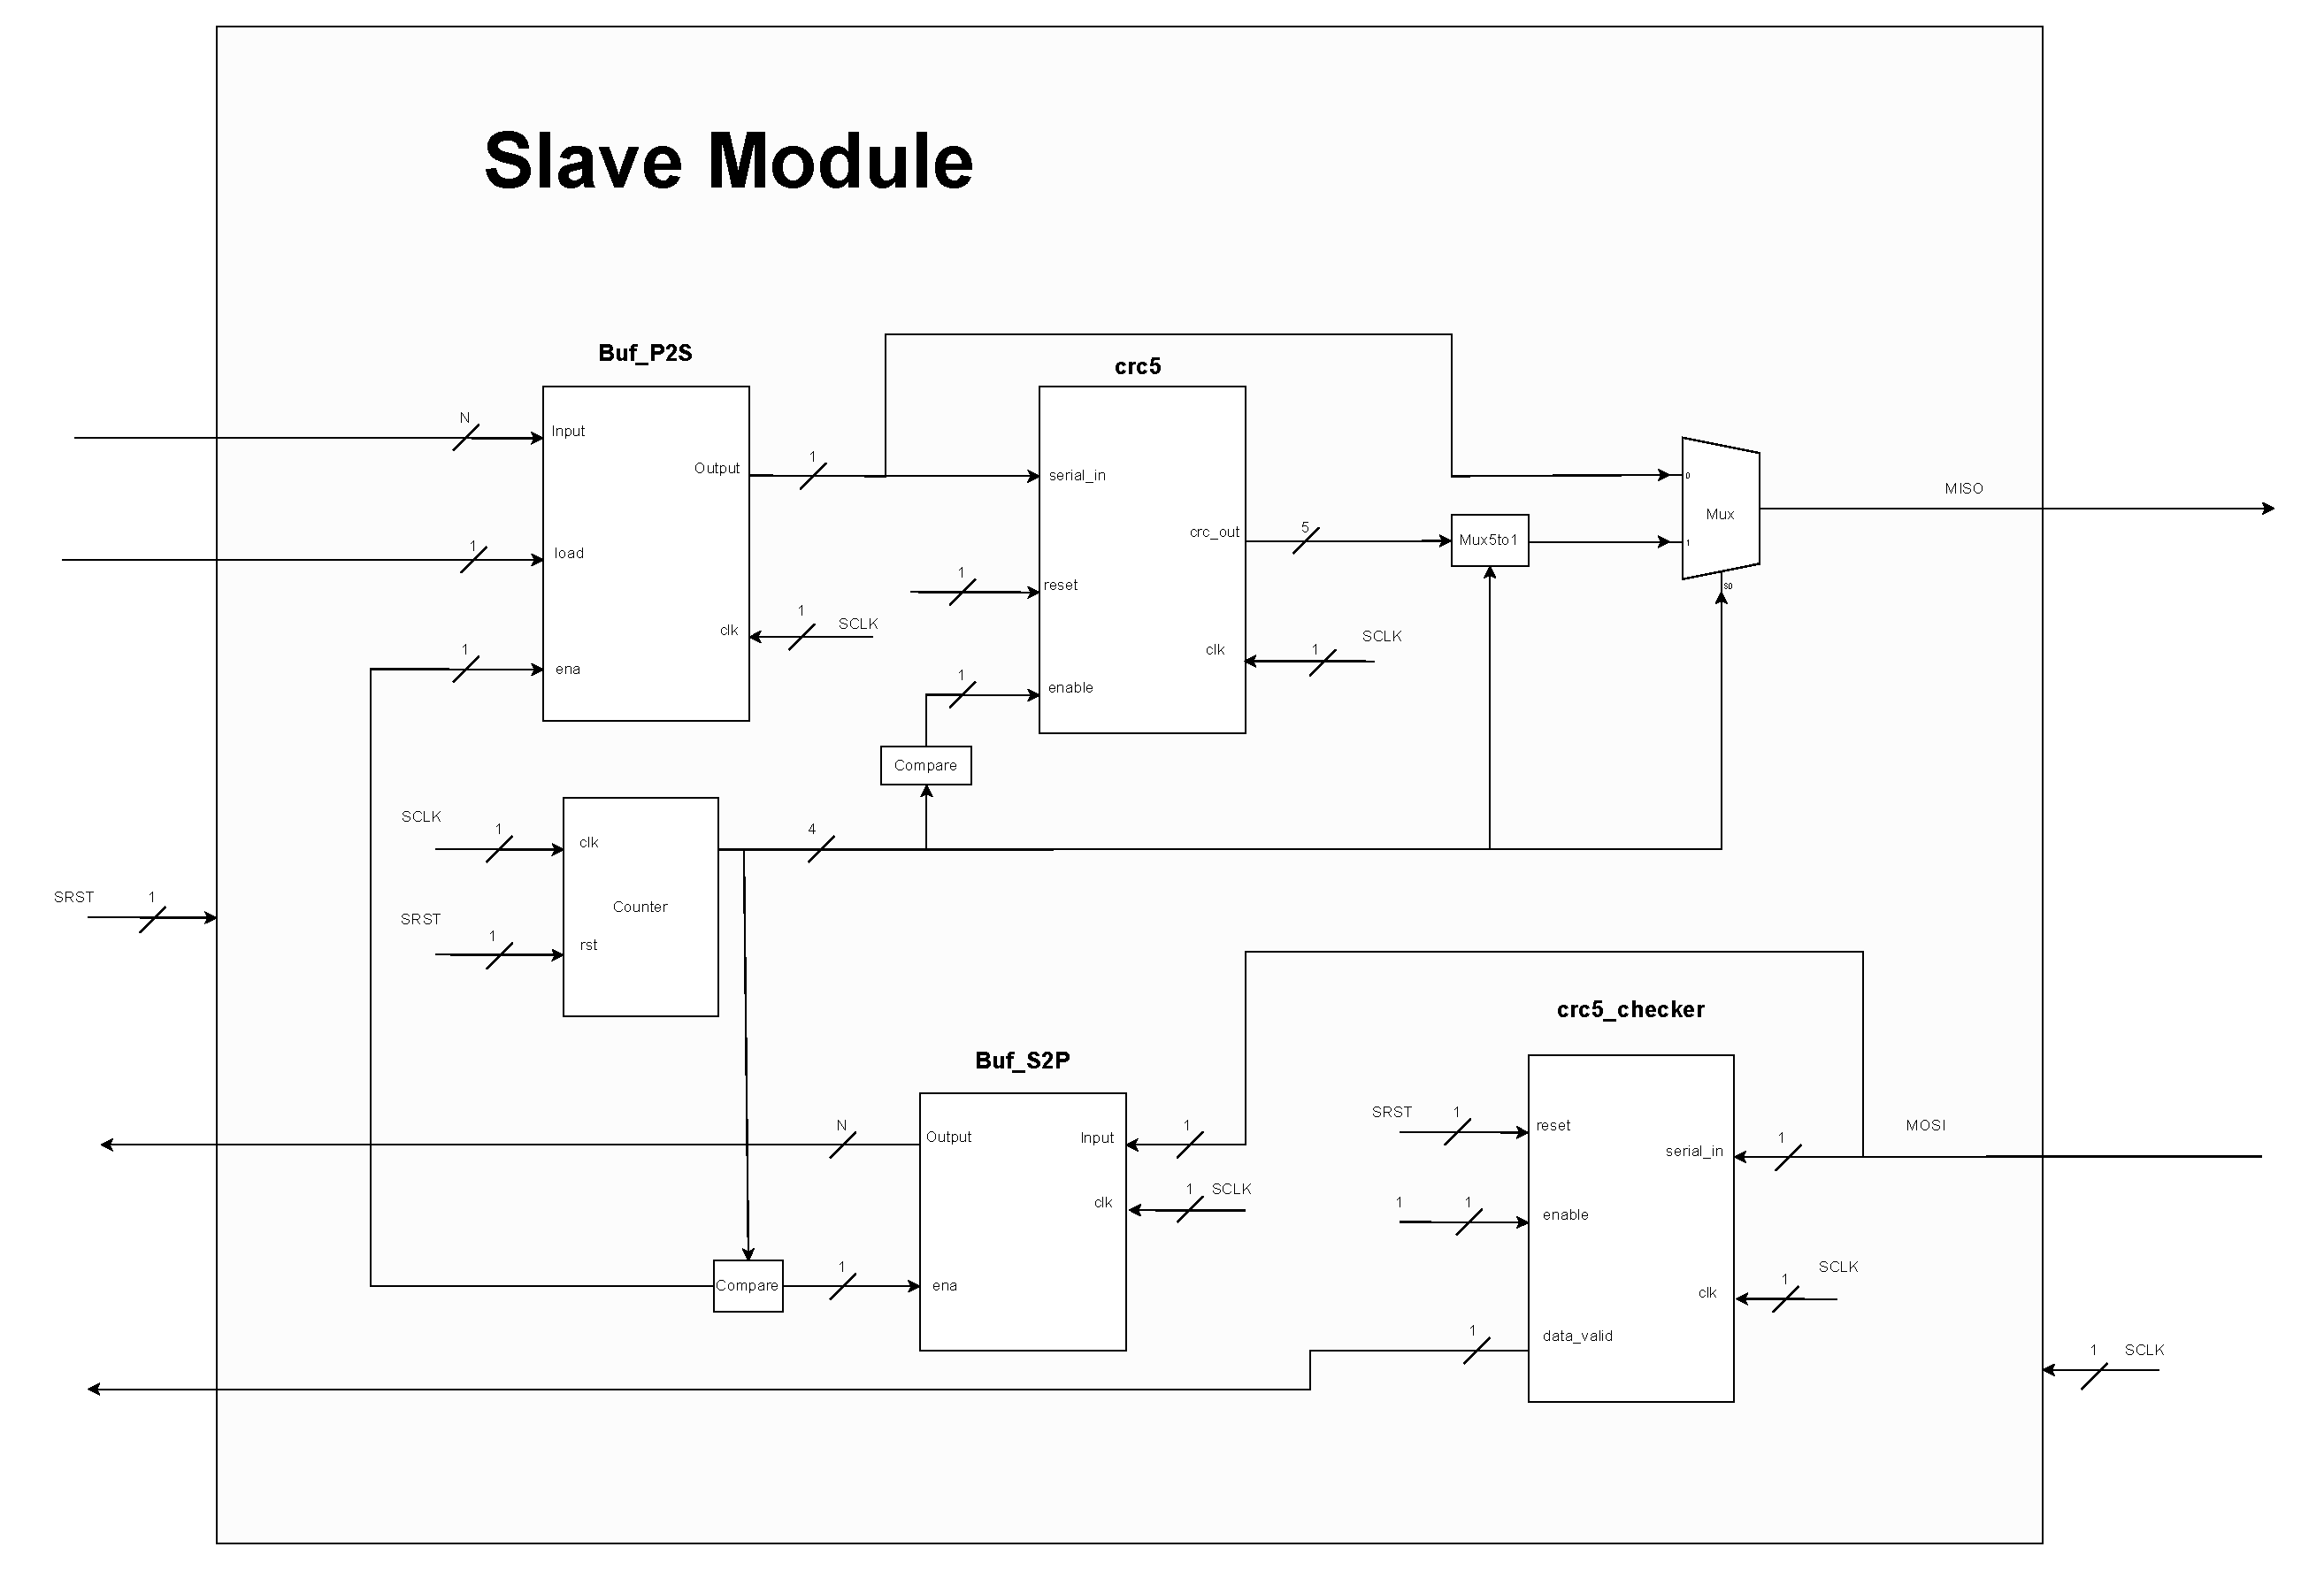
\includegraphics[width=0.85\textwidth]{graphics/Tai_6.pdf}
	\caption{Sơ đồ tổng khối Slave}
	\label{fig:slave_top}
\end{figure}
\subsubsection*{SPI\_Slave\_CRC}
\textbf{Tham số:} \texttt{n=8}, \texttt{crc\_len=5}, \texttt{total\_len=n+crc\_len}, \texttt{cnum=4}, \texttt{CPOL=0}, \texttt{CPHA=0}.\\
\textbf{Cổng vào:}
\begin{itemize}
	\item \texttt{n\_rst}: reset chủ động mức thấp.
	\item \texttt{data\_in[n-1:0]}: dữ liệu song song từ Slave đưa ra MISO.
	\item \texttt{load}: nạp dữ liệu vào bộ P2S.
	\item \texttt{sclk}: xung SPI từ Master.
	\item \texttt{MOSI}: dữ liệu nối tiếp từ Master.
	\item \texttt{n\_cs}: chip select chủ động mức thấp.
\end{itemize}
\textbf{Cổng ra:}
\begin{itemize}
	\item \texttt{data\_out[n-1:0]}: dữ liệu nhận được sau khi gom đủ N bit.
	\item \texttt{MISO}: dữ liệu nối tiếp trả về Master (bao gồm data và CRC).
	\item \texttt{rx\_data\_valid}: báo dữ liệu nhận hợp lệ (CRC đúng).
	\item \texttt{rx\_done}: báo đã nhận xong khung (data+CRC).
	\item \texttt{crc\_out[crc\_len-1:0]}: CRC của dữ liệu phát ra.
	\item \texttt{ready}: báo Slave sẵn sàng truyền/nhận.
\end{itemize}

\subsubsection*{Parallel\_to\_serial}
\textbf{Chức năng:} chuyển dữ liệu song song \texttt{data\_in[n-1:0]} sang chuỗi bit \texttt{data\_out} khi \texttt{load} và \texttt{ena} được kích hoạt.

\subsubsection*{serial\_to\_parallel}
\textbf{Chức năng:} thu dữ liệu nối tiếp \texttt{data\_in} thành từ song song \texttt{data\_out[n-1:0]} khi \texttt{ena} hoạt động.